\documentclass[]{article}

\usepackage{graphicx}
\usepackage{listings}
\usepackage{wrapfig}
\usepackage{color}

\graphicspath{ {./images/} }

\definecolor{dkgreen}{rgb}{0,0.6,0}
\definecolor{gray}{rgb}{0.5,0.5,0.5}
\definecolor{mauve}{rgb}{0.58,0,0.82}

\lstset{frame=tb,
	language=Java,
	numbers=left,
	numberstyle=\scriptsize,
	aboveskip=3mm,
	belowskip=3mm,
	showstringspaces=false,
	columns=flexible,
	basicstyle={\small\ttfamily},
	numbers=none,
	numberstyle=\tiny\color{gray},
	keywordstyle=\color{blue},
	commentstyle=\color{dkgreen},
	stringstyle=\color{mauve},
	breaklines=true,
	breakatwhitespace=true
	tabsize=3
}

\lstdefinelanguage{json}{
	basicstyle=\normalfont\ttfamily,
	numberstyle=\scriptsize,
	stepnumber=1,
	numbersep=8pt,
	showstringspaces=false,
	breaklines=true,
	frame=lines,
	literate=
	*{0}{{{\color{mauve}0}}}{1}
	{1}{{{\color{mauve}1}}}{1}
	{2}{{{\color{mauve}2}}}{1}
	{3}{{{\color{mauve}3}}}{1}
	{4}{{{\color{mauve}4}}}{1}
	{5}{{{\color{mauve}5}}}{1}
	{6}{{{\color{mauve}6}}}{1}
	{7}{{{\color{mauve}7}}}{1}
	{8}{{{\color{mauve}8}}}{1}
	{9}{{{\color{mauve}9}}}{1}
	{:}{{{\color{dkgreen}{:}}}}{1}
	{,}{{{\color{dkgreen}{,}}}}{1}
	{\{}{{{\color{delim}{\{}}}}{1}
	{\}}{{{\color{delim}{\}}}}}{1}
	{[}{{{\color{delim}{[}}}}{1}
	{]}{{{\color{delim}{]}}}}{1},
}

\lstdefinestyle{ascii-tree}{
	literate={├}{|}1 {─}{--}1 {└}{+}1 
}
%opening
\title{Relazione progetto Reti WORTH
\large https://github.com/fulviodenza/worth}
\author{Fulvio Denza, 544006, f.denza@studenti.unipi.it}


\begin{document}

\maketitle

\section{Introduzione}
WORTH è un modo per condividere il workflow di un progetto. Esso rappresenta una delle metodologie AGILE che si sono sviluppate negli ultimi anni. Il modello di WORTH è un modello semplificato di applicativi del campo, quali easy redmine, trello e molti altri. In WORTH vediamo l'esistenza di una sequenza di stati dei vari task, quale todo, in progress, to be revised e done, la presenza di una chat per ogni progetto, azioni basilari sulle card (o task) quali change status, add card, get card history ed altre.

Il modus operandi per presentare i comandi del progetto sarà bilaterale, ossia verrà descritto l'azione del client e la risposta del server, mentre le strutture dati e le scelte di implementazione delle astrazioni saranno presentate nelle rispettive sezioni del server o del client.

\section{Package Server}
Il server contiene la logica del nostro applicativo, contiene le Classi per descrivere le componenti di WORTH, esso parte da una classe Main.
\subsection{Main}
Il main presenta le istanziazioni delle classi per la connessione TCP e per la RMI Callback
\begin{lstlisting}[language=java]
//Main.java
//REGISTER
UserRegister ur = new UserRegister();
Runtime.getRuntime().exec("rmiregistry 2020");
System.setProperty("java.rmi.server.hostname","0.0..0");
ur.RemoteHandler(5455);

//LOGIN
ServerNotification serverCB = new ServerNotification();
ServerNotificationInterface stubCB = (ServerNotificationInterface) UnicastRemoteObject.exportObject(serverCB, 0);
String name = "notification";
LocateRegistry.createRegistry(7001);
Registry registryCB = LocateRegistry.getRegistry(7001);
registryCB.bind(name, stubCB);
	
//TCP Connection
TCPConnection connection = new TCPConnection(serverCB);
connection.start(5456);
if(Thread.interrupted()) connection.stop();
System.out.println("Server Started");
\end{lstlisting}
Le righe di codice sopra riportate presentano semplicemente l'istanziazione delle classi Server per le nostre RMI Callback che verranno invocate nel momento in cui il client effettuerà una register e una login. La TCP Connection è il modo in cui viene istanziato il server TCP per aprire il canale di comunicazione lato server implementato per mezzo di una ServerSocket sulla porta 5456.\\
\begin{center}
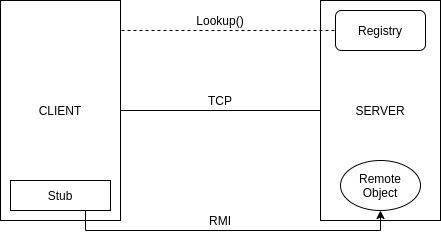
\includegraphics[scale=0.6]{classDiagram}
\end{center}
\subsection{Database}
\begin{wrapfigure}{l}{0.25\textwidth} %this figure will be at the right
	\centering
	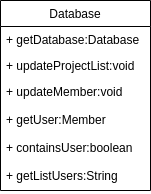
\includegraphics[width=0.25\textwidth]{databaseDiagram}
\end{wrapfigure}
Il database è stato sviluppato usando la libreria di Google gson, esso consiste in un file .json contenente tutti gli utenti nella forma:
\begin{lstlisting}[language=json]
n:
	username: "username"
	password: "password"
	projectList:
		0: "project"
		1: "project"
		...
\end{lstlisting}
in cui n è l'indice, nel file json, della posizione dell'utente, il campo username e password sono i campi in cui vengono conservati le relative informazioni, projectList contiene, invece, la lista di progetti a cui appartiene l'n-esimo utente.
Una miglioria, nonchè best practice, sarebbe potuta essere implementare un algoritmo di crittografia per salvare le password cifrate, anzichè in chiaro, tuttavia ai fini del progetto non era strettamente necessario.\\
Il database contiene i campi
\begin{lstlisting}[language=java]
private static volatile Database database;
private static Path dbFile;
private static final ConcurrentHashMap<String, Member> db = new ConcurrentHashMap<>();
\end{lstlisting}
Ho dichiarato Database database volatile perchè avevo bisogno di una garanzia per il database che il suo valore sia uguale ovunque, sia nella cache sia nella memoria principale affinchè non ci siano problemi di lettura/scrittura qualora consumassero o producessero il database più thread alla volta,
la variabile database contiene la struttura stessa del database.
la ConcurrentHashMap db contiene le associazioni (Username, Member) che verranno usate per le ricerche su database, ogni qualvolta la ConcurrentHashMap viene modificata, viene modificato anche il database.json. È stata scelta una struttura dati concorrente in modo da gestire gli accessi dei Thread, questa scelta migliora sensibilmente le performace del nostro applicativo.
\paragraph{getDatabase}
getDatabase è il metodo usato per usare il database esistente o, se non esistente, crearne uno nuovo.
\paragraph{updateMember}
updateMember è il metodo per aggiornare il file json degli utenti del database.
\paragraph{updateProjectList}
updateProjectList server per aggiornare la lista dei progetti a cui l'utente indicato nei parametri è iscritto.
\paragraph{getUser}
getUser è il metodo getter per ottenere dal file database.json l'utente che come username ha quello indicato tra i parametri. Il metodo effettua una ricerca sulla ConcurrentHashMap del database rispetto alla chiave String username.
\paragraph{containsUser}
containsUser è il metodo per restituire una risposta alla domanda: "l'utente si trova nel database?". Questo metodo usa la getUser per capire per effettuare la ricerca, se il metodo getUser non throwa un'eccezione MemberNotFoundException, restituisce true, altrimenti false.
\paragraph{getListUser}
Il metodo getListUser viene usato per restituire una stringa contente tutti gli utenti separati, nella stringa, da un carattere speciale \$ e ogni utente è descritto da una coppia username:status
\subsection{CardStatus, Card, Project}
CardStatus è l'enum per definire gli stati in cui si può trovare una Card, Card, a sua volta, è la definizione di una Card come data nelle specifiche, Project è la composizione delle Cards, in Project vengono definite svariate strutture per organizzare le card.
\begin{center}
	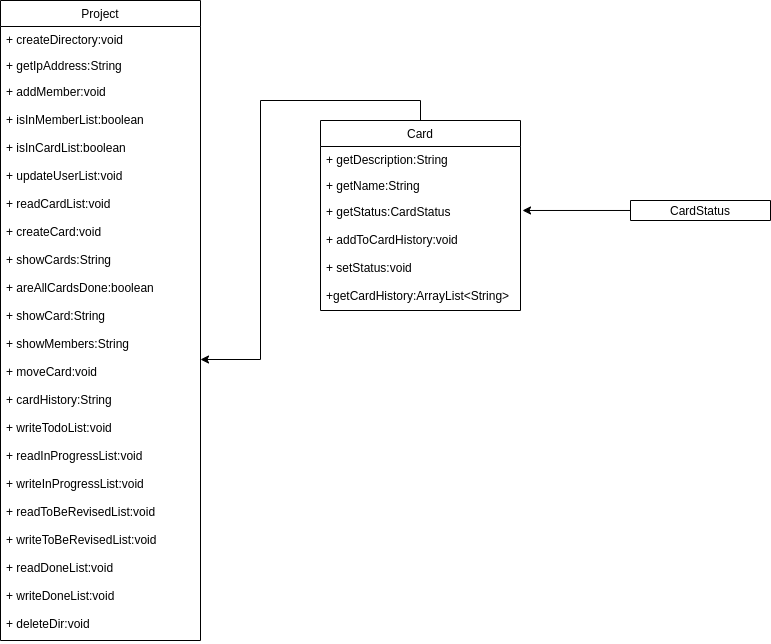
\includegraphics[width=1\textwidth]{architecture}
\end{center}
\subsubsection{CardStatus}
CardStatus è un semplice enum che contiene i possibili stati di una Card:
\begin{itemize}
	\item TODO
	\item IN\_PROGRESS
	\item TO\_BE\_REVISED
	\item DONE
\end{itemize}
\subsubsection{Card}
Card è l'elemento fondamentale di ogni Progetto, una Card è un task, un pezzo di lavoro che si trova in una certa situazione tra quelle descritte in CardStatus. Una Card ha 4 campi principali: 
\begin{lstlisting}[language=java]
private String name;
private String description;
private CardStatus status;
private ArrayList<String> cardHistory;
\end{lstlisting}
i primi 3 sono autoesplicativi, il quarto, cardHistory, è la lista di Stati che ha attraversato la carta in questione.
Ognuno di questi campi ha un metodo getter, mentre hanno un metodo setter status e description. Il metodo addToCardHistory è il metodo utilizzato per aggiornare la Card.
\subsubsection{Project}
Project è la classe più grande del progetto WORTH. Essa contiene tutta la logica relativa ai progetti all'interno di WORTH.
\begin{lstlisting}[language=java]
public String projectName;
public ArrayList<String> memberList;
public ArrayList<Card> taskList;
public ArrayList<Card> TODO_List;
public ArrayList<Card> IN_PROGRESS_List;
public ArrayList<Card> TO_BE_REVISED_List;
public ArrayList<Card> DONE_List;
\end{lstlisting}
Ogni Status possibile ha una lista associata, in aggiunta a questi abbiamo una taskList, ossia la lista di tutte le Card in un progetto, memberList, ossia la lista dei membri di un progetto e, ovviamente, projectName, il nome identificativo del progetto.
Il metodo costruttore di Project non è altro che l'istanziazione delle varie liste, rappresentate da $Arraylist<String>$ che contengono semplicemente i nomi delle varie Card presenti nel singolo Progetto e la creazione dei file per ogni singola lista, in modo da garantire la persistenza.
La struttura di una cartella progetto è questa:
\begin{lstlisting}[style=ascii-tree]
	projects/
	└── project
	├── cards.json
	├── done.json
	├── in_progress_list.json
	├── to_be_revised.json
	├── ip_address.json
	├── memberList.json
	└── todo_list.json
\end{lstlisting}
Oltre a questo, il metodo costruttore contiene anche la generazione di un ip usando il metodo statico
\begin{lstlisting}
public class IPGenerator {
	public static String generateIPAddress() {
		
		return (ThreadLocalRandom.current().nextInt(224, 239+1) + "." + ThreadLocalRandom.current().nextInt(0, 256) + "." + ThreadLocalRandom.current().nextInt(0, 256+1) + "." + ThreadLocalRandom.current().nextInt(0, 256+1));
	}
}
\end{lstlisting}
Il quale, con la classe ThreadLocalRandom, genera una stringa composta da 4 parti separate da un punto, ogni parte rappresenta una porzione di indirizzo IP partendo da 224.0.0.0 e finendo all'indirizzo 255.255.255.255, ossia il subset di indirizzi utilizzabili come indirizzi multicast.
\paragraph{createDirectory}
Il Metodo createDirectory è composto da un if$\cdot$else per descrivere l'esistenza o meno del progetto nella directory dei progetti. Quindi, se non esiste il progetto, viene creata la cartella e il file con, all'interno, l'ip address, altrimenti stampa a schermo "Project exists in the project folder"\\
Da adesso, molti metodi saranno della forma:
\begin{lstlisting}
Gson gson = new Gson();
BufferedReader br;

try {
	File f = new File(path+"/file.json");
	if(!f.exists()) {
		f.createNewFile();
	}
	br = new BufferedReader(new FileReader(path+"/file.json"));
	Type type = new TypeToken<InterestedType>() {
	}.getType();
	dataStructure = gson.fromJson(br, type);
} catch (IOException e) {
	e.printStackTrace();
}
return dataStructure;
\end{lstlisting}
per la lettura aggiornata del contenuto di file.json e il suo salvataggio in 
$$<InterestedType> dataStructure$$
al fine di utilizzare la versione aggiornata del file json e,
\begin{lstlisting}
Writer writer;
try {
	writer = new FileWriter(path+"/file.json");
	Gson gson = new GsonBuilder().setPrettyPrinting().create();
	gson.toJson(dataStructure, writer);
	writer.flush();
	writer.close();
} catch (IOException e) {
	e.printStackTrace();
}
\end{lstlisting}
per la scrittura di dataStructure in file.json.\\
Questi due metodi verranno utilizzati in coppia per deserializzare e serializzare una qualsiasi struttura dati di cui avremo bisogno in futuro.
I due metodi sono l'equivalente di una update dataStructure e update file.json, una che scrive nella struttura dati e una che scrive nel file json.\\
I metodi della prima forma (\textbf{Reader}) sono:
\begin{itemize}
	\item readCardList, per salvare nella struttura dati dell'oggetto Project la lista di Cards;
	\item readTodoList, per salvare nella struttura dati dell'oggetto Project la lista di Cards nello stato TODO;
	\item readInProgressList, per salvare nella struttura dati dell'oggetto Project la lista di Cards nello stato IN\_PROGRESS;
	\item readToBeRevisedList, per salvare nella struttura dati dell'oggetto Project la lista di Cards nello stato TO\_BE\_REVISED;
	\item readDoneList, per salvare nella struttura dati dell'oggetto Project la lista di Cards nello stato DONE.
\end{itemize}
I metodi della seconda forma (\textbf{Writer}) sono:
\begin{itemize}
	\item updateCardList, per rendere persistenti i cambiamenti effettuati nella struttura dati taskList;
	\item writeTodoList, per rendere persistenti i cambiamenti effettuati nella struttura dati TODO\_List;
	\item writeInProgressList, per rendere persistenti i cambiamenti effettuati nella struttura dati IN\_PROGRESS;
	\item writeToBeRevisedList, per rendere persistenti i cambiamenti effettuati nella struttura dati TO\_BE\_REVISED;
	\item readDoneList, per rendere persistenti i cambiamenti effettuati nella struttura dati DONE.
\end{itemize}
Un miglioramento che si sarebbe potuto fare sarebbe stato creare un singolo metodo per ogni tipologia (Writer e Reader) in cui si indicava la struttura dati e il file da Scrivere o Leggere, in modo da non avere ripetizioni di codice.\\
Abbiamo poi dei metodi ausiliari 
\begin{itemize}
	\item getIpAddress, per restiture l'ip address dal file json, andando a prendere l'ip dal file ipAddress.json;
	\item isInMemberList, per restituire la risposta alla domanda "l'utente è nella lista utenti del progetto?" andando a controllare in memberList.json;
	\item isInCardList, per restituire la risposta alla domanda "la card è nella lista di cards del progetto?" andando a controllare nel file cards.json;
	\item addMember, per aggiungere un membro nella struttura dati e aggiornare il json all'ultima versione della struttura dati;
	\item createCard, per creare una nuova card e alla fine dell'operazione aggiornare il json all'ultima versione della struttura dati.
	\item showCards, per restituire una stringa contente tutte le cards separate da un carattere speciale \$;
	\item areAllCardsDone, per effettuare una visita al file cards.json e controllare se tutte le cards siano nello stato DONE, se lo sono, restituisce true, altrimenti restituisce false;
	\item showCard, per cercare la card con il cardName dato nel parametro, effettua una visita per controllare che quella card ci sia e in tal caso restituire una stringa della forma:\\
	NAME:name\$STATUS:status\$DESCRIPTION:description,
	ossia i campi descrittivi della card richiesta che sarà manipolata dal client.
	\item showMembers, per restituire una stringa della forma:\\
	member1\$member2\$...\$memberN,
	ossia la lista di membri appartenenti a un progetto, che sarà poi manipolata dal client.
	\item moveCard, infine abbiamo la move card che segue il seguente automa:
	\begin{center}
		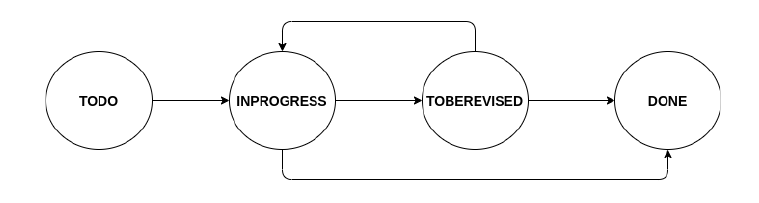
\includegraphics[scale=.5]{graphStatus}
	\end{center}
	La moveCard contiene il seguente algoritmo: per ogni operazione ammissibile, legge il file json in cui si trova la card e ne salva il contenuto nella struttura dati, effettua la rimozione dalla struttura dati, scrive la struttura dati aggiornata nel json, legge il file json di destinazione (indicata dall'utente) e ne salva il contenuto nella struttura dati, ne aggiunge la Card, se esiste, e carica il contenuto della struttura nel file json interessato.
\end{itemize}
\subsection{TCPConnection e ConnectionHandler}
Il server, come abbiamo visto nel main, istanzia l'oggetto TCPConnection e "starta" il thread.
Lo fa istanziando una ServerSocket presso la porta indicata nel main e, all'interno di un ciclo infinito, istanzia un oggetto Thread che istanzia una ConnectionHandler, passandogli come parametri serverSocket.accept() e serverNotification, questi due parametri serviranno al gestore della connessione per mandare sulla socket le risposte ai comandi invocati dal client e la serverNotification per utilizzare la Callback RMI per inviare la lista di utenti ONLINE e OFFLINE presenti nel sistema.\\
Sulla serverSocket il server riceverà il comando mandato dal client conservandolo nell'array \textit{command}, l'array command avrà nella posizione 0 il comando stesso, nella posizione 1 conterrà i parametri del comando stesso, separati da un ":".
In questa implementazione \textit{command[0]} verrà inserito all'interno di uno switch...case per gestire ogni singolo comando che arrivi al server e all'occorrenza verranno separati i parametri di \textit{command[0]} in ogni case a seconda di quanti parametri il \textit{command[0]} prenda.\\
Torneremo dopo su ogni case al fine di capirne meglio l'implementazione dei comandi.
\subsection{RMI: ServerNotification e UserRegister}
\paragraph{UserRegister} La classe UserRegister viene usata per gestire il comando di registrazione dell'utente ed implementa i metodi dell'interfaccia. \\Per l'implementazione del metodo register ho creato un Registry sull'host presso la porta 5455 e ho bindato il nome "RegisterUserInterface" all'oggetto UserRegister, in modo che fosse localizzabile dal client. Il metodo register non fa altro che aggiungere l'utente al file database.json se l'utente con il nome utente inserito dal client non esiste già, altrimenti skippa l'azione stampando "SERVER: user already registered!".
\paragraph{ServerNotification} La classe ServerNotification viene usata per gestire il servizio di notifica degli utenti e del loro stato. ServerNotification ha un campo $List<ClientNotificationInterface> clients$ e un campo $List<String> usersList$, il suo metodo costruttore è semplicemente l'istanziazione di queste due liste. Quando si effettua una chiamata al metodo register, si iscrive semplicemente il client al servizio di notifica aggiungendolo alla lista e si aggiunge la stringa relativa al suo username alla lista di Stringhe, quando si effettua una unregister si rimuove il client e la stringa relativa al suo username dalle liste relative.
sendMemberList effettua una singola chiamata al metodo doCallbacks il quale, a sua volta, genera un iteratore di clients e finchè questo iteratore non giunge al termine, istanzia un oggetto della classe ClientNotificationInterface client ed effettua una chiamata al metodo notify di quest'ultima classe.\newpage
\section{Package Client}
\end{document}
